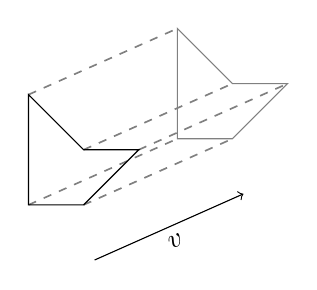
\begin{tikzpicture}[scale=0.7]
\draw[->, shift={(2.2,0)}] (0,0) -- (2.7, 1.2) node[pos=.5, sloped, below] {$\vv{v}$};
\draw[gray, dashed, semithick, shift={(1,1)}] (0,0) -- (2.7, 1.2);
\draw[gray, dashed, semithick, shift={(2,1)}] (0,0) -- (2.7, 1.2);
\draw[gray, dashed, semithick, shift={(3,2)}] (0,0) -- (2.7, 1.2);
\draw[gray, dashed, semithick, shift={(2,2)}] (0,0) -- (2.7, 1.2);
\draw[gray, dashed, semithick, shift={(1,3)}] (0,0) -- (2.7, 1.2);
\draw (1,1) -- (2,1) -- (3,2) -- (2,2) -- (1,3) -- cycle;
\draw[gray, shift={(2.7,1.2)}] (1,1) -- (2,1) -- (3,2) -- (2,2) -- (1,3) -- cycle;
\end{tikzpicture}
